\documentclass[a4paper,11pt]{report}
\usepackage{graphics}
\usepackage{color}
\usepackage{epsf}
\usepackage[pdftex]{graphicx}
\usepackage{subfigure}
\usepackage{setspace}
\usepackage{cite}
\usepackage{makeidx}
\usepackage{footmisc}
\usepackage{url}
\usepackage{multicol}

\usepackage[T1]{fontenc}
\usepackage[sc]{mathpazo}
\renewcommand{\ttdefault}{cmtt}
% \linespread{1.05}         % Palatino needs more leading (space between lines)


\addtolength{\textwidth}{\oddsidemargin}
\addtolength{\textwidth}{\evensidemargin}
\addtolength{\textwidth}{-1cm}
\addtolength{\textheight}{1.5cm}
\setlength{\oddsidemargin}{0.5cm}
\setlength{\evensidemargin}{0.5cm}
\setlength{\topmargin}{0in}

\bibliographystyle{apalike2}
% TODO: \emph stuff
%TODO: Spanning Tree To Correct Language
\begin{document}

\begin{titlepage}
 
\end{titlepage}

\begin{abstract}
 
\end{abstract}

\tableofcontents

\chapter{Introduction}

\chapter{Background}

There has been a great deal of work in compression over the years, however, there is very little research on compressing Molecular Dynamics data specifically.
The following sections will describe various background necessary to an understanding of our approach.
Section \ref{back_mdf} describes the most dominant format that is used for storing the simulations on hard disk,
while sections \ref{back_intra} and \ref{back_inter} describe various techniques used in the related field of video compression.

\section{Molecular Dynamics Formats}
\label{back_mdf}

There are several Molecular Dynamics Simulations formats. Chief among these formats is the binary DCD file. This is the principle format used in Visual Molecular Dynamics(VMD)\cite{vmd}, a popular program for visualisation of molecules and simulation. This format also relies heavily on an existing PDB file in order to make sense of the output.

The PDB file stores information about each specific atom in the simulation. This generally includes the atom's element and the atom's group, the latter only important for use in protein simulations.[Possibly a reference here?] The data in the PDB file is stored in ASCII so the file is often larger than necessary. However, the PDB file only stores information for each atom and not for each frame in the simulation, so we are less concerned about the size of this file. A large amount of information is redundant when using DCD files: The PDB file stores positions for each atom, which are ignored when a DCD file is loaded. The main reason for the redundant information is to enable the molecules to be viewed in its normal state using just the PDB file and nothing else.

\subsection{DCD format}
The DCD format has various types which all differ slightly from each other. These differences may be ignored for most purposes as they normally store extra information in the header of the DCD file. VMD is able to handle all major variants such as the CHARMm and X-PLOR formats, however the main format used is the X-PLOR format. \cite{vmddcdformat}

All these types have very slight differences which are mainly for keeping information about the original simulation, for instance the timestep between each frame. The DCD file format does not specify a prefered endian representation. The endianess of the data can be identified by magic numbers stored in the header, but any system that allows for loading DCD files must be able to handle both little and big endian correctly. The header also contains information relating to the number of atoms and the number of frames in the simulation.

The majority of the file is dedicated to storing the frames of the simulation. Each frame of the file indicates a single timestep in the simulation. In each frame the positional information about each atom is stored. The positions are stored as triples of x, y and z 4-byte single precision floating point numbers. This makes up the majority of the file, as each atom repeated in every frame requires 12 bytes to fully specify. The order of the atoms in the frame is important as they correspond to the order of the atoms in the PDB file. No further information is stored in the file after the end of the final frame. The size of the final file can be estimated using the formula: 

\begin{center} $size = 12*frames*atoms$ bytes\end{center}

The above formula is only an estimate as it does not account for the header. Another problem is that in certain format types there can be atoms which remain fixed in space for the duration of simulation. These atoms are only stored in the first frame rather than in all frames. It is reasonable to ignore these effects in the majority of simulations as they typically only account for a fraction of the original atoms. [TODO: Incorporate John Stone email to next thing] Molecular simulations may have millions of atoms stored at each step and can involve many thousands of frames. This can result in files that are several gigabytes in size and in extreme cases, several terabytes in size.

These simulations need to be archived so that they can be reviewed by a molecular biologist at a later date or   they may need to be transmitted over slow media such as network connections. Given their large size, it is often necessary to use compression.

\section{Molecular Simulation Compression}
\label{back_msc}
To date, there has been little research on compressing large-scale molecular dynamics simulations. The current method\cite{RefWorks:3} for compression is able to acheive output sizes smaller than the original by an order of magnitude. The method does not have any specific name, so for the remainder of this report we will refer to it as Omeltchenko's algorithm. There are two other algorithms of note that are useful for this situation. These are the Gandoin \& Devilliers Algorithm[TODO: cite] and the Predictive Point Cloud Compression Algorithm[TODO: cite]. Both of which are used for compressing point cloud data. A point cloud is a collection of points, where each point has position and possibly other attributes. Atoms stored in a PDB file may be treated as a point cloud.

\subsection{Omeltchenko's Algorithm}


[TODO: This is not really true since they refer to compressing atoms as a whole, instead of only the positions. They compress the positions, velocities and any other information.]

The algorithm works by quantising the space that the simulation occurs in. This space is usually taken to be the axis-aligned bounding box that encompasses all the atoms, which has to be recalculated on a per-frame basis. A three dimensional grid of a particular granularity is embedded into the space. Atoms are snapped to the centers of the closest grid cell. This transformation introduces a small error, which can be controlled by the granularity of the grid, but enables the algorithm to reduce the floating point coordinates to integer-based grid cell indices. This step, known as quantisation, is commonplace in point compression. It allows insignificant variations in the data to be removed, while introducing a quality setting to allow for better compression at the cost of accuracy. This stage produces a quantised (x, y, z) coordinate for each atom. As a post operation, the points are translated so that all coordinates are non-negative.

The atoms indices are mapped to Octree Indices. An Octree is a spatial partitioning data structure, which recursively splits space up into 8 subdivisions. The subdividing process typically stops when there are few points in a cell or a maximum depth has been reached. A related variant of Octrees is Linear Octrees, where the data structure is represented in a 1D array. Octree Indexing is a reversable spatial hashing algorithm where 3D points are mapped to 1D indices, by using the Linear Octree cells. In this case, the quantised points are mapped to single non-negative integers. The algorithm uses Octree Indexing to interleave the bits of the coordinates of each point. The index, itself, is cleverly assembled so that points are only interleaved up to the largest most significant bit of every coordinate.

\begin{figure}
 \center
 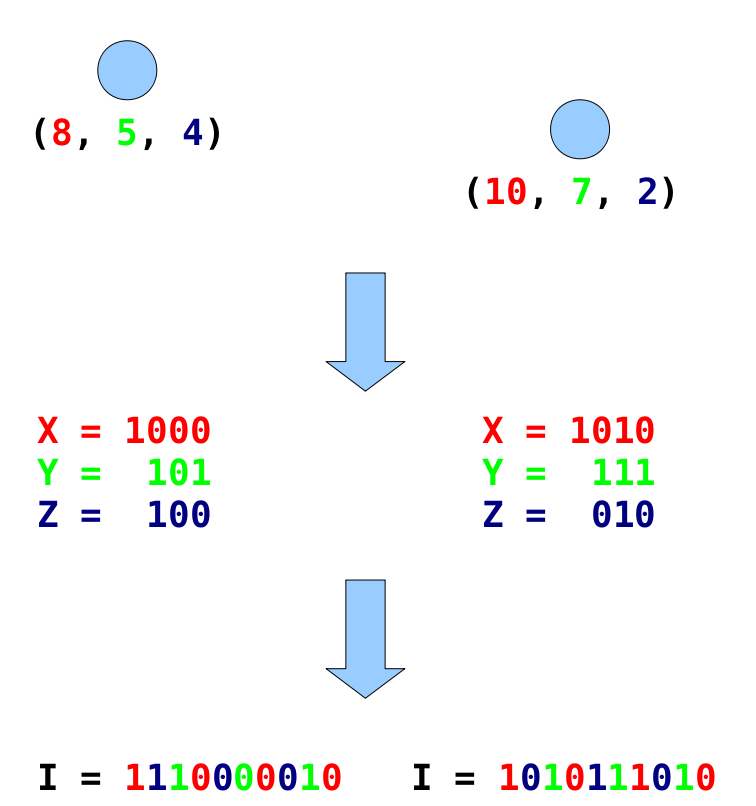
\includegraphics[width=0.4\textwidth]{resources/OctreeIndexingVerticalCropped.png}
\caption{Demonstration of the Octree Indexing Process on a system of 2 atoms.}
\label{octree}
\end{figure}

The resulting indices are stored in a list and sorted in increasing order. These indices are written to the file using a delta encoding scheme. The first atom's position indicates its actual grid index, while the rest are stored as differences between the previous index and the current one. This final transformation typically allows a better compression rate to be acheived. Delta encoding reduces the amount of data that needs to be compressed by keeping things small, however it introduces a dependancyThe output, itself, is performed by an adaptive, variable-length compressor. Typically, each index can be stored in a single 4-byte integer which results in an immediate size reduction from 12-bytes per atom to 4-bytes per atom. 

The compressor encodes the molecular data as a series of non-negative integers. Each integer streamed into the compressor one at a time. The compressor maintains an integer $l$ which is the current size that integers are encoded as. As each integer comes into it is checked to see if the integer can be stored using $l$ bits. If it can, it is stored as $l+1$ bits; a 0-bit followed by the bits of the integer. If it can't, the integer is partly stored as $l+1$ bits; a 1-bit followed the first $l$ bits of the integer. The rest of the bits are compressed in the next step of the compressor. When enough of these overflows occur, $l$ is incremented.

The compressor was designed to be very computationally light as computers at the time of the paper were not as powerful as current machines. The paper claims that 56-byte atomic data is encoded at approximately 6.3 bytes per atom. It is, however, not considered to be a very good compression system as it is not based on any of the established variable-length encoders which have been shown to produce near-optimal encodings.

The paper does not use the common file formats such as those used in VMD, it does however treat atoms very similarly so we are able to use the scheme for DCD file compression. The algorithm deals with atoms that are represented by a block of 56-bytes, containing position(24-bytes), velocity(24-bytes) and an ID(8-bytes). In our application, the atoms are defined only as 12-byte position data, but have an implicit ordering from the PDB file. Since the sorting destroys the ordering, additional information will need to stored to recover the initial ordering when decompressing.

\subsection{Gandoin \& Devilliers' Algorithm}

The Gandoin \& Devillier's Compression Algorithm exploits a property of KD trees[TODO: cite] to compress Point Cloud Data.\cite{devillers2000gci} A KD tree is a spatial subdivision data structure which partition space using various axis-aligned splitting planes. The KD tree cycles through each dimension for the splitting axis as the data structure is recursively constructed. The splitting planes are chosen to divide the space in half each time.

The algorithm exploits the property that if one knows the number of points over the entire space and the number of points in one of the regions that were created from the split, one can work out the number of points for the other region by simple arithmetic.

Each leaf node of the tree is subdivided if there are multiple points in the region. The points in the compression are usually quantised. The original frame may only have distinct points, however the quantised frame could have several duplicates depending on the quality of the quantisation. For this reason, the subdivision might stop before the number of points in a cell is less than 2.

An advantage of this algorithm is that it is progressive. This means that low-detail representations of the point cloud can be constructed from the initial parts of the compressed stream. As the compression progresses the detail in the model becomes finer until the output reaches the final quantised result. This algorithm produces a symbol stream which is usually encoded with an entropy encoder such as Arithmetic Coding.[TODO: cite]

\subsection{Predictive Point Cloud Compression Algorithm}

Predictive Point Cloud Cloud Compression is a new approach to compressing point cloud data. The compression scheme creates a spanning tree of the original point set using heursitics.\cite{gumholdcomp} Predictors based on these heuristics exploit patterns in the data to get an estimate of the position of a child in the tree relative to its parent. The use of these predictors means that only the residual error from each prediction needs to be stored.

In the original paper the algorithm only used one of two predictors for the entire models to encode the entire pointset. The user was prompted for which predictor to use. The first predictor predicted that the child would be placed in the same position as the parent, while the second predictor estimates the child to be the same displacement as the displacement between its grandparent and parent. Further enhancements to the algorithm were made to choose the best predictor at each step of the algorithm and also extra predictors were added.\cite{merrycomp}

The performance of this algorithm depends greatly on the quality of the predictors used. Poor predictors will result in significantly worse compression. The compression scheme requires the number of small errors to be high which decays very rapidly as the the error size increases. The predictors also require that the point cloud represent a surface so that information such as the surface normal at each point can be estimated.

\section{Video Compression}

A different approach is to follow that of video compression. Essentially, the molecular simulations can be viewed as videos, but using 3D dimensional molecular data instead of 2D picture data. We can safely ignore the audio part of compression as it bears no importance on molecular simulations. Video Compression loosely falls into one of two subcategories. The first is intraframe compression which seeks to compress each individual frame using little or no information about previous frames. The other type is interframe prediction which uses a significant amount of information from previous frames to compress a frame. 

Usually, each frame is heavily analysed for objects that are considered important. These objects are often major features such as a person's arm or a ball. The purpose of the intraframe compression is to record these objects with their initial positions, while interframe predictions estimates the position of the objects and only records the errors that occur from making the estimate. In most cases, given a good predictor, the error is usually small and can be compressed very well.

The rest of this section will discuss the algorithms used in both intraframe compression and interframe prediction. The techniques used to detect objects in the images are ignored as our simulations have atoms which are clearly defined objects.

\subsection{Intraframe Compression}
\label{back_intra}

The latest MPEG encoding algorithms allow for several compression algorithms to be used\cite{gall1991mvc}. This section will focus on the most common algorithms used for compressing the objects in the original image. These algorithms can be classified as either lossless or lossy. Lossless compression algorithms are able to recreate the original data with no loss of information. These lossless compression algorithms are general enough to apply to standard data compression. Lossy compression algorithms, on the other hand, are able to achieve much higher compression rates, but do incur the penalty of some information loss. Typically, the lossy compression algorithms only quantise the input to fit within a certain number of symbols and still require further compression from a lossless algorithm. We will focus mainly on the lossless compression techniques as information loss, aside from small quantisation errors, may result in incorrect assumptions being drawn from simulations.  

In the remainder of the chapter we will discuss only the lossless compression techniques. These techniques fall into two categories: Entropy encoders and dictionary encoders. 

\subsubsection{Entropy Encoders}

Entropy encoding makes use of Information Theory and tries to build an optimal mapping from symbols in the frame to individual bits. In a video frame, this information could be lossily compressed blocks of pixel data or information about identified object. In a molecular simulation we could easily use this to store positions of molecular data.

The first such algorithm was called Huffman Encoding\cite{citeulike:1320251}. The original Huffman Encoding relies on having frequencies of all symbols that occur in the message to be compressed. It uses this table to build up a prefix-free tree. A prefix-free tree's leaves are symbols and the paths from the root to a leaf indicates the bits required to output that symbol. The frequencies allows the algorithm to construct an `optimal` tree which requires less bits to output common symbols and more bits to output rare symbols. Decoding a single symbol from a message  entails following the paths indicated by the bits until a symbol is reached, or looking up the bitpatterns in a table.

\begin{figure}
 \center
 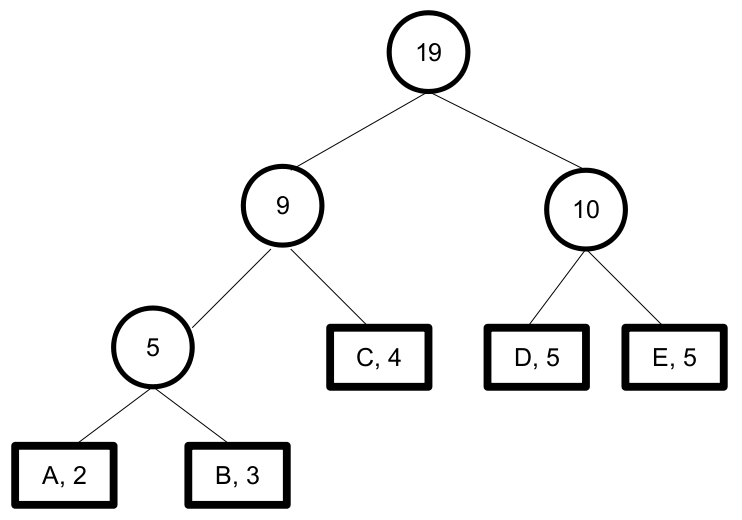
\includegraphics[width=0.4\textwidth]{resources/HuffmanTreeCropped.png}
\caption{Huffman Tree for a simple alphabet of \{A,B,C,D,E\} with given frequencies.}
\label{huffman}
\end{figure}

There are various issues when using regular Huffman Encoding. The first problem is that the entire message must be available when we write the compressed data in order to compute the frequency table.\cite{RefWorks:1} The second problem is that in order to decompress we need to also output all the prefix-tree used to compress. These problems can be remedied by Adaptive Huffman Encoding\cite{42227} which is able to re-optimise the prefix-tree while the compression occurs.

The Adaptive Huffman Encoding scheme is a good candidate for compression of the molecular simulation frames. The memory footprint of the algorithm is low, only the prefix-free tree needs to be stored while the algorithm runs and has a worst-case space usage of $O(S)$, where $S$ is the number of unique symbols in the frame. The algorithm can also be run while the simulation takes place as only a small amount of computation needs to occur per atom.

There is a similar entropy-based compression algorithm called Arithmetic Coding. This algorithm has an advantage over Huffman Encoding as it can store symbols as a fractional number of bits. \cite{RefWorks:1}, \cite{RefWorks:3}. The amount of wasted bits that appear in Huffman Encoding can be as bad as 1 bit per symbol. Arithmetic Coding works by encoding the entire message into a single rational number in the range [0, 1). The frequency of each symbol is used to allocate large subranges to frequent symbols and small subranges to rare symbols. 

\begin{figure}
 \center
 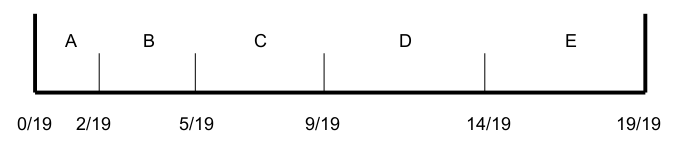
\includegraphics[width=0.8\textwidth]{resources/ArithmeticCoder.png}
\caption{Arithmetic Coder ranges for same alphabet in Figure \ref{huffman}}
\label{arithmeticcoder}
\end{figure}

Encoding a specific symbol simply requires adjusting upper and lower bounds of the output number. When the entire message is encoded the number can be output. Decoding simple requires one to follow the subranges that the encoded message falls into.

\begin{figure}[h]
 \center
 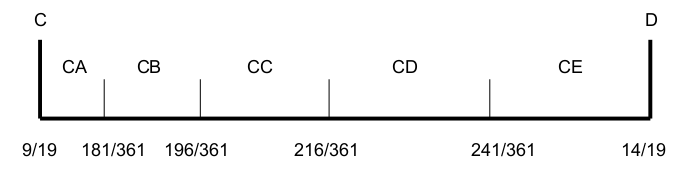
\includegraphics[width=0.8\textwidth]{resources/ArithmeticCoderSubrange.png}
\caption{Arithmetic Coder ranges after encoding a C}
\label{arithmeticcodersubrange}
\end{figure}

Arithmetic Coding implementations are typically very complex. Some implementations use a static dictionary of 256 symbols, while others are able to handle only up to a dynamic dictionary of up to a few thousand symbols. The reason for this is that the numbers for the ranges are not implemented using an arbitrary precision rational number library. Instead they use a representation based on regular 32-bit integers. Overflow and underflow issues are handled by scaling the range.

Unfortunately, there are problems with the original arithmetic algorithm in that you need to compute the entire frequency table which needs to be output before any compression can begin. The Adaptive Arithmetic Coding algorithm is an adjustment that does not require the frequency table to be constructed, but it does, however, require that symbols are stored prior to the output number. 

Both the Adaptive Arithmetic Coding algorithm and the Huffman Coding algorithm require a separate component for handling the frequency table. Unlike, the regular static algorithms, this frequency table needs to allow insertion of new symbols, updating the frequencies of existing symbols as well as determining which symbol a given frequency belongs to and what the frequency range of a symbol is. Two common data structures for storing this data structure are arrays and Fenwick Trees.
%The two most common data structures for this are range trees[TODO: cite] and Fenwick trees[TODO: cite].

In most implementations, the core Arithmetic Coding encoding algorithm is separated from the static or adaptive parts of the algorithm. The core algorithm is usually called the encoder and decoder, as it is only responsible for encoding and decoding ranges. The encoding and decoding part is independant on whether one uses the adaptive or static algorithm. The parts of the algorithm that handle the adaptive and static part is calleod the model. This separation allows for better modularity and design of an arithmetic coder.

The Arithmetic Encoding scheme offers a better choice for compression of the frames. The adaptive models allow us to update symbol frequencies while the frame is being compressed. This leads to the same worst-case space usage as Huffman Encoding. The adaptive algorithm also requires only a small amount of computation per symbol. However, the problem remains of conveniently storing the symbols for each output file.

\subsubsection{Dictionary Encoders}

Dictionary-based encoding schemes attempt to compress data using a different approach from entropy encoders\cite{RefWorks:2}. A data structure known as dictionary is able to efficiently keep track of a sliding window of text information. This window allows different dictionary encoding algorithms to take advantage of distributions of symbol placement data in the input message. Rather than using frequencies as a basis for shorter codewords, they resort to greedily assigning symbols or groups of symbols to codewords of increasing length. This gives certain advantages over entropy encoders, such as being fast and requiring little or no mapping information necessary to decode the data. 

There are various dictionary-based compression algorithms, key among them are the LZW and DEFLATE algorithms. The LZW algorithm keeps an explicit dictionary that is progressively built up as the stream is read.\cite{1320134} Using this information, a codeword for the current symbol can be worked out and written to file. This algorithm needs to store additional information with the text in order to reconsitute the initial dictionary, but after this the message can recreated by dynamically updating the dictionary. 

The DEFLATE algorithm uses several techniques such as an additional layer of Huffman Coding for bit-reduction, a sliding window based dictionary and a duplicate string removal algorithm\cite{deflaterfc}. It is the most commonly used dictionary-based compression algorithm and is used in applications such as gzip and in the PNG image format. 

Dictionary-based encoding schemes tend to perform worse on average than entropy-based encoders, but can perform much better for certain messages, for instance, where there are large runs of repeated information. Dictionary-based encoding schemes require very little computation per symbol and have low memory overheads. However, these overheads can be larger than in entropy encoders. 

% \subsubsection*{Vector Quantisation}
% 
% Vector Quantisation is a common technique used in video and speech compression systems.\cite{RefWorks:1} The mechanisms, by themselves, do not compress the algorithm, but instead attempt to reduce the number of unique symbols that are used in the frame. This output is then used as input for a lossless compression scheme such as Huffman Encoding. Vector Quantisation algorithms acheive this symbol-reduction by considering the symbols to exist in some N-dimensional vector space. This space is then split up into various cells whose identifiers will be used as the symbols to compress. The mapping from symbols to cells must also be stored in the compressed output.
% 
% The first algorithm for creating the cells is known as Lloyd-Max algorithm.\cite{108235} The iterative algorithm creates a Centroidal Voronoi Diagram. A Centroidal Voronoi Diagram is a subdivision of N-dimensional space into $L$ cells. Each cell has exactly one point assigned to it, which is the centroid of each cell, and the cell is defined as the volume of space which is closest to the cell's point. The centroidal property keeps the information lost in the transformation at a minimum.\cite{RefWorks:1} The algorithm's complexity increases exponentially as the dimension of the space increases which makes it infeasible in even low dimensions.\cite{116880}
% 
% The second algorithm for creating the cells is the K-means algorithm.\cite{1979} This is an iterative algorithm which differs from the Lloyd-Max algorithm by using the mean of the cells instead of the centroid. This adjustment negates the need for a Voronoi Diagram and thus it often outperforms the Lloyd-Max algorithm, however the quality of the cells generated is a trade off.
% 
% These algorithms are only slightly applicable to the domain of molecular compression. The first trade off that we have made is the loss of information in the simulation. This is countered, however, by being able to acheive a much higher compression rate than lossless encoders. They also need an entire frame of information in order to run and thus lead to a higher memory usage. They can also be infeasible to perform alongside a molecular dynamics simulation.
% 
% \subsubsection*{Transform Coding}
% 
% Transform coding is another group of image compression algorithms which attempt to reduce the detail present in a frame. They are suited towards images due to the large amount of numerical information that allows the transformation to occur. These transformations are typically followed by a lossless encoding scheme.
% 
% The first such transform was the Discrete Fourier Transform\cite{Cody92thefast}. This algorithm transforms the digital signals, the pixels, into analogue signals which represent the image. These signals can be analysed using a frequency analysis. The signals have different effects on the image. Lower frequencies determine the large scale structure of the image, while higher frequencies are responsible for detailed parts of the image. A function called a convolution, in this case a low-pass filter is applied to cut off any high frequencies, reducing the detail in the image.\cite{1464352} The Discrete Fourier Transform was later replaced with the Discrete Cosine Transformation, as Discrete Fourier Transformations tend to perform worse around the borders of the image\cite{RefWorks:1}.
% 
% Transform coding is a commonly used lossy compression scheme in image and video compression. However, the same problems as with Vector Quantisation occur. It requires an entire frame to be streamed in before any compression can begin. It will also perform poorly in molecular simulations because we are compressing a atom point list instead of a volume of space. They also require slightly more computation than regular lossless encoding schemes.

\section{Interframe Prediction} 
\label{back_inter}

Interframe prediction takes advantage of the correlation between the current frame and previous frames. Objects that are identified are predicted to be in a new position. Most of the time, the prediction will be incorrect, but, if the predictors are chosen carefully, the predicted position will be close to the actual position. If the errors are small, they can be effectively compressed, using an entropy encoder, as individual errors are likely to occur more frequently. There are several types of prediction that is used. We will discuss, specifically, first-order prediction, K-th order prediction and Kalman Filtering.

There are several noticable differences with the prediction schemes used in standard video formats and the molecular dynamics simulations. The first difference derives from the fact that these schemes require some information to bootstrap the prediction. Frames in molecular dynamics simulations can use positions of the atoms in previous frames to predict on, while videos often only have pixels. The latest compression schemes break the video up into blocks. Objects are identified within these blocks. Prediction can the be performed on the objects giving a high rate of compression. The MPEG-4 format specifies a single prediction scheme with a large number of features\cite{wiegand2003oha}. 

A related topic is that of index frames. One of the reasons this prediction is not used completely throughout a video file is that it makes every frame in the file dependant on all the frames that precede it. In order to decode a frame in the file, every prior frame must be decoded. To allow for random access in a video, certain frames are labelled as Index frames or I-frames which are compressed only using Intraframe compression. Typically, a structure called a Group Of Pictures will be given that defines the order of the I-frames, and predicted frames, or P-frames\cite{vandalore2001sal}. There are also frames that can predicted from the previous or the following frames, called B-frames. This structure is useful to have in any compression scheme for molecular dynamics simulations to allow for random access in the simulation using both intraframe and interframe compression.

\subsubsection{First Order Predictors}

First order predictors use the current velocity of an object as a predictor to where the object will appear in the next frame. The velocity is calculated as the difference of the between the positions of the object in the previous two frames. This scheme would be particularly easy to implement in a molecular dynamics simulation where objects are explicitly given.

The error is coded as the difference between the predicted and actual position of the object. Given the physical nature of the simulations, this error is likely to be small, however, in a normal video there can be situations where this predictor does not perform very well.

\begin{figure}[h]
 \center
 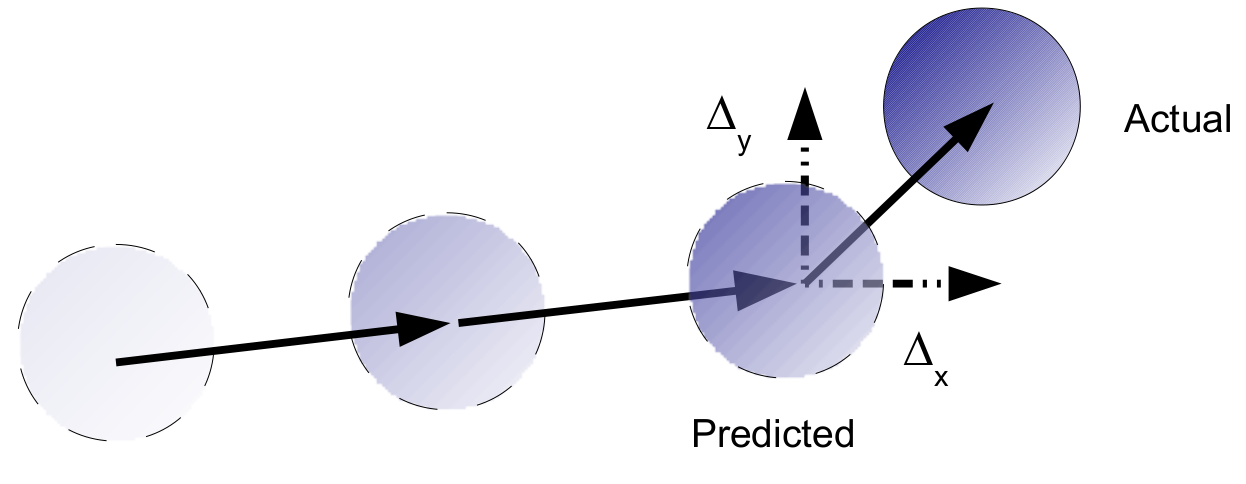
\includegraphics[width=0.6\textwidth]{resources/FirstOrderEncoding.png}
\caption{First Order Encoding of a point}
\label{linearencoding}
\end{figure}

\subsubsection{K-th Order Predictors}

K-th order predictors are an enhancement of the first order predictor by instead of just the positional data of the last two frames, they use object's positional data of the last $K+1$ frames to calculate the first $K$ derivatives of the object's position. Essentially, what is been calculated is a curve that passes through all $K+1$ previous positions. These predictors are updated when the next frame is encoded and used to predict the next position of the object.

\begin{figure}[h]
 \center
 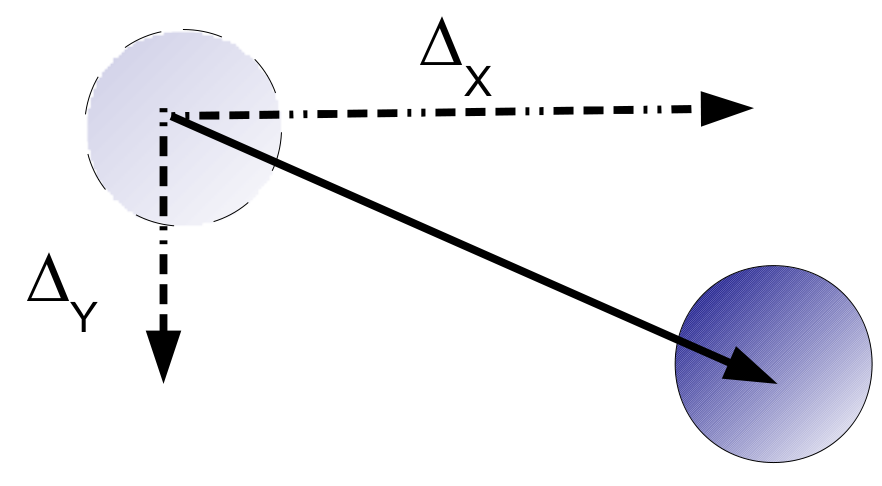
\includegraphics[width=0.6\textwidth]{resources/DeltaEncoding.png}
\caption{0-th order Encoding of a point, also known as delta encoding}
\label{deltaencoding}
\end{figure}

The error is again coded as the difference between the predicted and actual position of the object. However, there are several drawbacks to using K-th order predictors. The positional data of each of the objects must be kept from the previous $K+1$ frames. Also, each prediction requires $O(K^2)$ work to be performed per object. Another problem is that as $K$ increases, the quality of the predictions need not necessarily increase, and could even decrease resulting in large error rates.



\subsubsection{Kalman Filtering}

Kalman Filters are a relatively advanced prediction system that represent the motion of an object as a stochastic process.\cite{welch1995ikf} The predicted position at timestep $k$, $p_k$, of the object can be simulated as a linear stochastic difference equation of the form:
\begin{center} $p_k = Ap_{k-1} + Bu_{k-1} + w_{k-1}$  \end{center}
The actual measurement data, $x$, is related to the current predicted state by:
\begin{center} $x_k = Hp_k + v_k$ \end{center}
$w_k$ and $v_k$ are random variables which are normally distributed which are related to the noise that occurs within the stochastic process. $A$ is a matrix relating the previous prediction to the current prediction. $B$ is a matrix relating optional control input, for instance additional prediction information. $H$ is a time-dependant matrix which relates the current prediction to the current actual measurement. The Kalman Filtering process adjusts the matrices within the equations to get better and better approximations of the motion of the object.

Kalman filters provides increasingly better predictions as more frames are encoded. The drawback is that several matrix multiplications are required to acheive this accuracy, which can be computationally expensive to do on a per-object basis. This is especially true in large scale molecular dynamics simulations where there could be millions of atoms. This extra computation, however, could have a dramatic impact on the rate of interframe compression due to the very small error rates.

\section{Summary}

There are two main techniques for compressing videos. Intraframe techniques reduce each frame to a collection objects, in molecular simulations these are the atoms, which are encoded using either entropy encoders or dictionary encoders. Entropy encoders include the techniques of Huffman Coding and Arithmetic Coding. Huffman Coding uses an algorithm to construct a prefix-free tree to map symbols to bits, but can waste up to $1-bit$ per symbol. Arithmetic Coding is a more complicated technique which uses rational numbers to encode symbols. Arithmetic Coding can encode symbols as a fractional number of bits, avoiding the wastage that exists in Huffman Coding.

Interframe techniques use temporal coherence to better encode each frame, however it introduces a dependence on some of the previous frames. Interframe compression attempt to guess the next state of objects and encode any errors. If the predictions are accurate, a better compression rate can be acheived. There were two main techniques that were investigated. First order and K-th order prediction compute curves that fit through a window and extrapolate from this curve. Kalman filters treat the motion as a stochastical process that can be estimated with some accuracy through the use of matrices.

\chapter{Design}

The project's main aim was to provide research into how effective certain methods of compression would be on molecular simulations. Our system was designed in order to test the effectiveness of the compression schemes. Using our system we could measure the performance of the compression methods, in terms of speed and size of the compressed file. The actual testing of the system would accomplished via scripting and not directly through our system.

\section{Design Methodology}

We settled for an iterative design methoodlogy. The system was designed so that the first iteration would have very little functionality, but still be able to compress simulations. The first iteration had only two compressors based on reference schemes working. The second iteration had more compressors, including schemes based on interframe prediction compressions. The third and final iteration had all the compressors and visualisation completed.

The initial design of the program was to have an integrated system that could handle compression, decompression and visualisation of the molecular simulation data. This was changed as we learnt that the compression would possibly be included in VMD. VMD allows the simulations to be visualised using several different representations and so our visualisation would not be useful for VMD.

The program was then split-up into components that could shared across multiple programs; the visualisation and the compressors. This was necessary as there was functionality that needed to be in both the visualisations and each compressor, such as quantising and dequantising points. The graphical front-end of the program would be handled entirely by Min-Young Wu, while the compression back-end would be split-up fairly between Keegan Smith and myself. 

Another motivation for splitting up the work load is that testing would require each part to be separated in order to more efficiently gather results. The final design was that the compressors would be able to run separately with a separate driver program for each one.

Another important design choice that was made was to separate the Interframe and the Intraframe compression schemes. In normal video compression schemes they are combined into a single scheme. In order to measure the performance of the interframe compression schemes it is necessary decouple them. The use of other schemes would make it difficult to measure the compression time and compression rate. 
 
The system was intended to be very memory efficient. As little memory would be used as possible in order to carry out the compression. Our main reason for this was that the data we were dealing with was very large. Individual frames were potentially several gigabytes in size. However, according to an email with John Stone[TODO: ref?] we were informed that the current state of the art in simulations had a much lower size limit of several megabytes. We settled for a design that was a lot less stringent on memory which simplified the implementation greatly.

The final requirements for the compression section of our system was that it would need to be able compress large simulations with large numbers of atoms and frames. We defined large simulations as consisting of at least:

\begin{itemize}
 \item $2,000,000$ atoms
 \item $10,000$ frames
\end{itemize}

From these requirements, we calculated that the size of each frame is only about $20MB$ at maximum. All of the intraframe compression schemes only require each frame once as they are being compressed, however the interframe compression schemes require a window of previous frames. Typically, this window is very small, so the impact of storing each frame in the window is negligble.

It is predicted that in the next 2 years, the state of the art clusters will be to create simulations containing between $10,000,000$ to $100,000,000$ atoms. In order to handle these increases our system may need to optimised in order to allocate as little memory as possible.


\section{System Overview}

\begin{figure}
 \center
 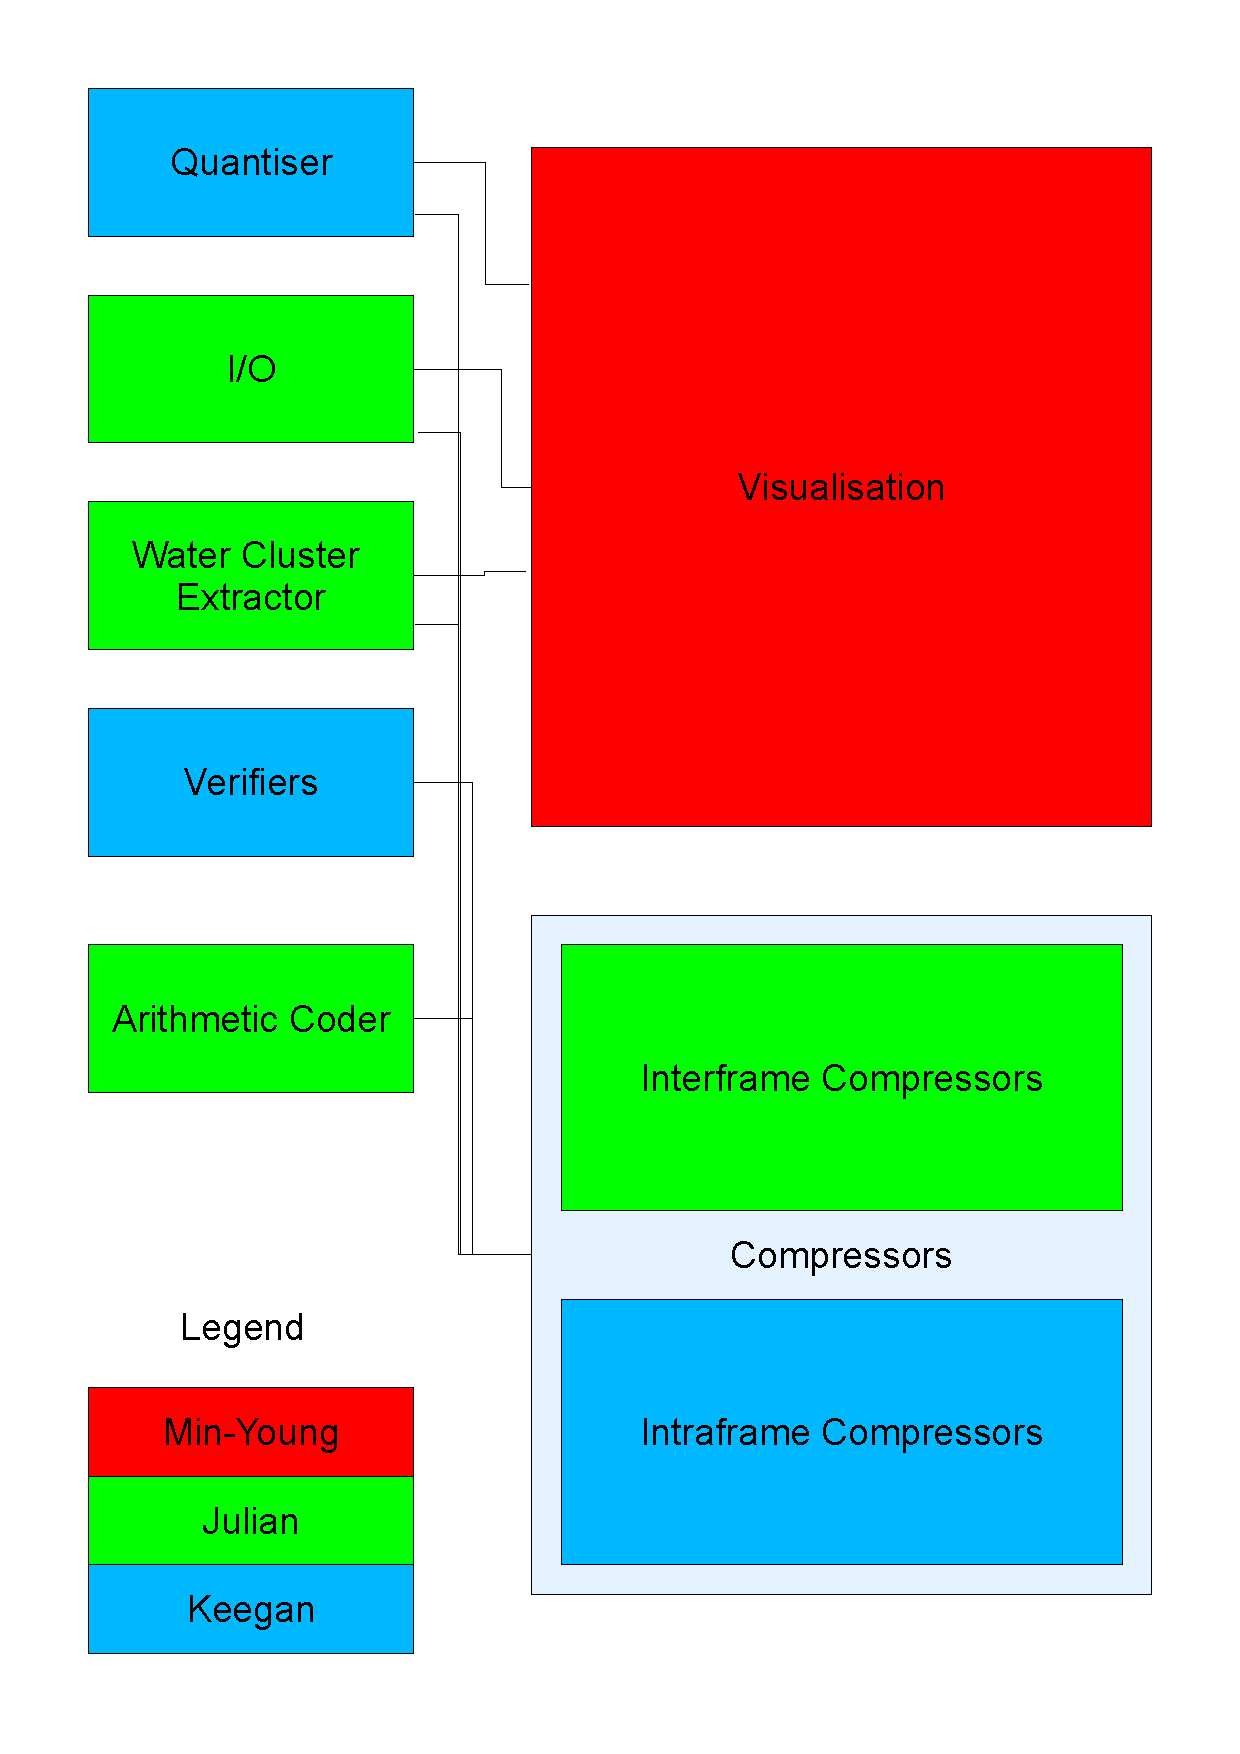
\includegraphics[width=0.4\textwidth]{resources/Breakdown-connect.pdf}
\caption{System breakdown}
\label{sysbreak}
\end{figure}

The system was divided up into several sections: Visualisation, Compressors and Components. The Visualisation handles viewing the output of molecular simulations that have been compressed by our system. It allows users to see the effects of quantisation on the simulations. This section was implemented by Min-Young Wu and is explained more thoroughly in his report. 

The Compressors section contains all the different compression techniques that were implemented. This compressors fall into one of two subsections: Intraframe and Interframe compression. The Intraframe compressors were mainly implemented by Keegan Smith, although the Omeltchenko Encoder was implemented by myself and its implementation will be explained later.

The Components part of the system represented various subsystems that are shared among various parts of the project. The main reason for separating these components out was to avoid code duplication. There were additional benefits such as easier testing and better splitting of the work load among our team.

The following is a list of the components and their roles in the systems. \\ \\ \\

\begin{itemize}
 \item Quantiser
 \begin{itemize}
   \item This component is responsible for the quantisation and dequantisation of the points in each frame of a simulation.
 \end{itemize}
 \item I/O
 \begin{itemize}
   \item These components performs I/O to and from the original DCD and PDB formats. 
 \end{itemize}
 \item Water Cluster Extractor
 \begin{itemize}
   \item The Water Cluster Extractor transforms the list of atoms into a list of water clusters and other atoms.
 \end{itemize}
 \item Verifiers
 \begin{itemize}
   \item These components verify the results of compression and gather statistics on the error in quantisation.
 \end{itemize}
 \item Encoder
 \begin{itemize}
   \item These components transform a list of symbols into a compressed bitstream.
 \end{itemize}
\end{itemize}


% This section will describe the design of the compression side of the project. The design of the visualisation aspect of the project is not described in this section as they are not necessary for measuring compression rates. The visualisation does, however, impact on some of the design choices required for the compression which are described in the appropriate sections.
% 
% To facilitate a well designed project, the compression aspect was split up into various components. These components act as transformations on input data, such as atoms in a frame, to produce required output data, for instance quantised atoms.

% These components are categorised in to several groups which relate to specific tasks that need to be accomplished. These groups are:



% Each of the components will be discussed briefly in the following section. Finally, there will be a discussion on the design of the experiments for recording the success of this method.

\section{Compressed File Format}

We chose a standard file format for all compressors to write to. This decision simplified the implementation of the compressors and easily allow adding new compressors in future. The format has several sections that allow it to reconstitute an uncompressed DCD file.

The header of the file is broken up into two segments. The first segment stores the DCD file's header which includes the number of atoms and frames in the simulation. The second segment stores header information relevant to the compression. In many of the compression schemes this is only the quantisation levels, however some of the interframe schemes require additional information about prediction window sizes.

The remainder of the file consists of records, one per frame. Each record contains a frame header followed by the compressed data. The frame header contains information about the bounding box of each frame. Using the bounding box and the quantisation levels, a quantised approximation to the original data can be constructed. The compressed data section is specific to each compression scheme.

\begin{figure}
 \center
 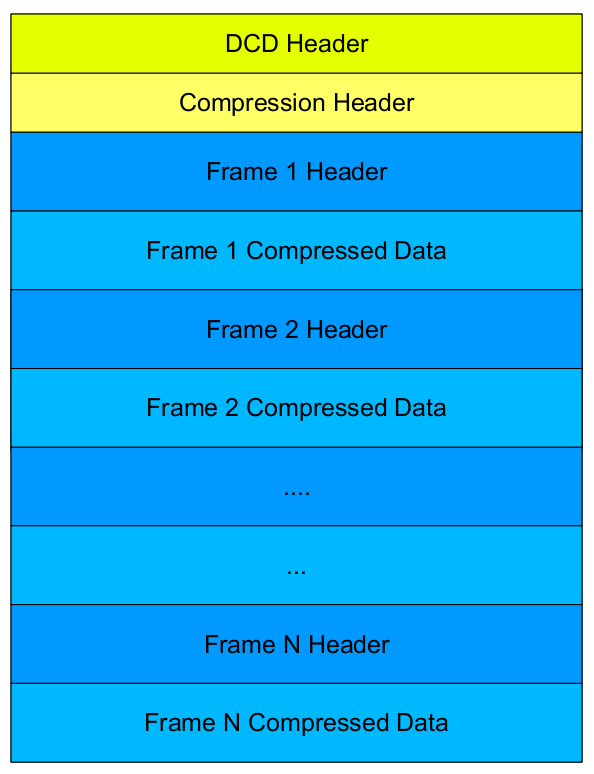
\includegraphics[width=0.4\textwidth]{resources/FileFormat.png}
\caption{File format}
\label{sysbreak}
\end{figure}

% \subsection{Overview}

\section{Experiment Design}

The experiments that are performed for evaluating the system are designed to test both compression rate and speed of the implementations. The important questions that we are requiring to ask is which compressor performs the best. [TODO: this is not really the question I set myself to answer in the proposal, I believe I only had to answer the question for Omeltchenko and Predictive Pointcloud Compression while Keegan Smith handled the Gandoin \& Devillier's and Predictive Pointcloud Compression]

The performance of the schemes will be compared by measuring the compression rate and speed on two levels. For each dataset the compression rate and computation time will be measured for each simulation in the entire dataset. Using this data, a mean running time per atom can be determined as well as the variation of these running times. Significant running times ocan point to issues that can cause the algorithms to perform slower. A similar argument can be made for the compression rate. The causes of high variation may be determined by looking at the number of water clusters in each frame in the case of Predictive Pointcloud Compression, while Omeltchenko may require further information to analyse.

Several datasets will be used. The sizes of the simulations will vary from very large, approximately one million atoms with one hundred to one thousand frames, to very small simulations of only a few thousand atoms and a few dozen frames, with several datasets in between. There will also be datasets that consist completely and of water and datasets that contain no water. Finally, we will also have datasets that contain a very complex molecule in solution.

\chapter{Implementation}

This chapter 




\section{Intraframe Compressors}

\subsection{Omeltchenko Scheme}



\section{Interframe Compressors}

\subsection{Polynomial Extrapolation}

\subsection{Common Error Encoding}

\subsection{Smallest Error Encoding}

\subsection{k-Nearest Neighbour Encoding}



\section{Quantiser}

The quantiser was implemented as a class which wraps around a vector. The class provides methods to convert to and from the normal unquantised frame. In order to easily incorporate the Omeltchenko scheme, it adjusts the points that are being quantised to be non-negative. Non-negative indices are required by the Octree Indexing method of the Omeltchenko scheme due to the bit-wise operations that must be performed.

Objects of this class store all the information necessary to 'dequantise' the points.

\section{I/O}

We chose to use the PDB and DCD file types exclusively as our target formats since these are the main formats used in VMD. We had separate components for each function we required from our project. 

\subsection{DCD I/O}

We used code from the VMD project for loading and saving of DCD files. This is mainly due to the DCD files have a complex binary format which is exacerbated by the unspecified nature of the endianess for each file. From reading the comments in the code we found that the loading of DCD files is not as efficient possible as it requires copying to separate buffers to reorder the coordinates in the atoms. We did not see this as a problem as it is mainly an issue with the DCD format. This does not impact the relative performance of each of our compressors as it adds a similar overhead to each file of the same size.

\subsection{PDB I/O}

Although there are many features of the PDB standard, only a very small subset of it is necessary. The PDB file is a text file that stores the data in several records. Our implementation of the PDB I/O only supports reading in of a PDB file. 

We also ignore any records which are not labelled ATOM. ATOM records store information regarding the type of each atom and what molecule it exists in, which is useful for detecting water molecules.

\subsection{Frame}

The frame component is simply a container that simply wraps a vector. It provides convenience methods that allow it to look more like a stream of floating-point atom coordinates.

\section{Water Cluster Extractor}

\subsection{Frame Splitter}

The Frame Splitting is used to break the atoms in a frame into two groups: Water molecules and non-water atoms. The splitting up is necessary for both visualisation and compression. The visualisation needs to know which atoms are water consitituients and which atoms are part of other molecules. 

On the compression side we also only need to  know which atoms form water molecules for the Predictive Point Cloud Compressor. Our implementation of the Frame Splitter requires that a valid PDB file be used in order to work correctly, so if the PDB is not available or not accessible, the Visualisation and Predictive Point Cloud Compressor will not work. 

There are various other implementations of the Frame Splitter that we could have tried which do not rely on the PDB file. In this implementation, we would assume that every atom was part of a water molecule and assign the bonds based on the two closest atoms. This was not implemented for two reasons. Firstly, the algorithm is likely to make incorrect assumptions about what the atoms are in the simulations. Secondly, VMD requires that a PDB file be loaded to view a DCD file so the required information is always likely to be available.

The algorithm to extract the water molecules uses a series of map data structures to connect the atoms into separate water molecules. The ATOM records collected from the PDB file are linearly scanned through. ATOM records with names other than ``OH2'', ``H1'' or ``H2'' can be safely categorised as not belonging to a water molecule. If the names do match, they are added to the maps.

\begin{figure*}[!h]
\begin{center}
 \small
 $map[atom\ name][residue\ name][residue\ sequence\ number][segment\ id] \rightarrow index into PDB file$
 \caption{The mapping system in order to determine the water molecule.}
\end{center} 
\end{figure*}

Using the STL map, this algorithm runs in average and worst-case time linearithmic time, however it could be improved to average case linear time using a hashtable-based data structure.

\subsection{Cluster Extraction}

The cluster extraction component's main job is to join water clusters into a clusters according to how these clusters form. Using the information from the Frame Splitter, the cluster extracter uses the polar nature of the atoms to predict where other water molecules in the same clusters are. Water molecules are connected if they are close to the predicted position.

[TODO: Pic]

The clusters, themselves, are stored as a graph data structure. The graph will have several components, one for each cluster. Edges between water molecules indicate a possible direct link between two water molecules. Although this may not be physically accurate, one can adjust a tolerance setting. A low tolerance will usually have lots of small water clusters consisting only of few water clusters. A high tolerance will have very few clusters which are a lot larger than they should be.

Since the core algorithm of the cluster extraction is a nearest neighbour lookup in a fixed radius, we tested two implementations. The first implementation used a 3-dimensional grid. The grid was implemented using the STL map data structure. The benefit of this was to decrease the space requirements for the grid. If a 3D array was used the memory usage could be quite large and grow with the size of the bounding box. Different methods of minimising the size of the grid by using coarser grid cells could have been used, but there are cases where the nearest neighbour lookup can degrade into a slower linear time operation. Using a map data structure allows one to have the size of the size of the data structure dependant only on the number of atoms and not the size of the bounding box. There is a drawback with this approach in that a cell look-up now requires logarithmic time, while the array method offers constant time cell look-up. The average case efficiency of this approach could be accelerated by using a hashtable based method or other spatial hashing method. The grid approach allows one to find the nearest neighbour to within a fixed radius by simple breadth-first search of the cells.

The other implementation used a library called Approximate Nearest Neighbour(ANN). [TODO: ref] ANN allows one to defer the task of nearest neighbour to a library. ANN typically uses one of two data structures to accomplish the searches: KD-trees and box-decomposition trees. The KD-trees discussed in [TODO: section] can also be used to find the nearest neighbour. The box decomposition tree uses various rules to decompose the space into a collection of boxes which cover the entire bounding box..



\section{Verifiers}

The verifiers were implemented as separate driver programs in the system. This separation allows the information to be collected without affecting the performance of the compression schemes. The verifiers can run after the compression and quantisation has been performed.

In our implementation we collect 4 statistics for each dimension separately.
\begin{itemize}
 \item Minimum Error: 
 \begin{itemize}
   \item The smallest difference between the original and quantised data.
 \end{itemize}
 \item Maximum Error:
 \begin{itemize}
   \item The largest difference between the original and quantised data.
 \end{itemize}
 \item Mean Error:
 \begin{itemize}
   \item The average difference between the original and quantised data.
 \end{itemize}
 \item Error Variance:
 \begin{itemize}
   \item The variance of the errors statistics between the original and quantised data. This is implemented using a linear algorithm after calculating the mean.
 \end{itemize}
\end{itemize}


\section{Encoder}





\section{Simulation I/O}

Components in this category handle the I/O of uncompressed simulation data. The required components required in this category are the DCD Reader/DCD Writer and PDB Reader.

\subsection{DCD Reader/DCD Writer}

The DCD Reader component is used to read the contents of the DCD file. This component must be able to handle special cases such as fixed atoms which are only stored in the first frame. The component must also allow random access into the DCD file on a per frame basis for visualisation purposes.

The DCD Writer component, on the other hand, is only required to write data out in a valid DCD format. This component needs access to the contents of the PDB so that the original order can be recovered.

\subsection{PDB Reader}

The PDB Reader component analyses the contents of the PDB file. The main purpose of this analysis is to determine which atoms correspond to Water molecules. There is no corresponding PDB Writer component as the PDB files are left unmodified by the compression schenmes. 

\section{Coders}

Coders are components which are able to encode symbols into a compressed form or decode a bitstream from a file into the original symbols. The components required are the Arithmetic Coder module and the Omeltchenko Coder module.

\subsection{Arithmetic Coder}

The Arithmetic Coder component is designed to be an Adaptive Arithmetic Coder that is able to handle sufficiently large numbers of symbols. This is crucial because the encoder must not only support the symbols required to decode the atoms, but also the symbols required to re-order the atoms correctly. Typically, Adaptive Arithmetic Coders are only able to handle a certain number of symbols with a certain maximum frequency, but for our uses we require that it must handle both an acceptable quantity symbols and high maximum frequency for large files.

\subsection{Omeltchenko Coder}

The Omeltchenko Coder component is designed as a simple adaptive encoder that is able to compress only integers. Data that is not in integer format, such as the ordering information is converted to an integer format first by using the information stored in the PDB file.

\section{Compressors}

These components facilitate the compression and decompression of the DCD files. They are `drivers` that are responsible for high-level file operations(opening and closing) and storing enough information to be able to reconsitute the original (quantised) DCD file. These components are objects which persist until the compression or decompression is complete. The components required are the Spanning Tree Compressor, Gandoin \& Deviller's Compressor and Omeltchenko Compressor.

Essentially the main purpose of these components is to be able to run the compressors without the need for any visualisation to be run simultaneously.

\section{General Components}

These components perform general transformations on the atom's in the simulation to produce an effect that is required for more than a single encoder. The components required in this section are the Interframe Prediction Coder, Frame Splitter and the Quantiser.

% \subsection{Quantiser}



% \subsection{Frame Splitter}



\subsection{Interframe Prediction Coder}

The Interframe Prediction Coder is used to reduce the running time of the compressors by using the temporal coherence of the simulation. Atoms in the simulation will likely not have deviated much from their original trajectory. The prediction scheme that will be implemented will be is a simple first-order scheme relying only on the two previous frames to get an estimate for the velocity.

There is one main complication, however, in that the specific implementation must be able to handle data of different dimensions. The Omeltchenko scheme produces 1D octree index data, while the other schemes do not require this. [TODO: ask if this is a good idea, or should we have the coder always output 3D coord differences]

\section{Method Specific Components}

This group contains components that are specific to only a single compression method. The required components are the Sorted Octree Indexer and the Delta Encoder/Delta Decoder for the Omeltchenko Algorithm,  Points To List Encoder for the Gandoin Algorithm and the Graph Creator, Spanning Tree Creator and Tree Serialiser for the Spanning Tree Compression Algorithm.

\subsection{Sorted Octree Indexer}

This component is responsible for computing the octree index of each atom in the frame. This component calculates the indices in the same way as described in the Omeltchenko paper. [TODO: cite]. A complexity that must handled is that we require the original order so we must store enough information with each index prior to sorting to recover this order. The input for this component is the output of the Quantiser component, while the output of this component is sent to the Delta Encoder component to be written out in a compressed form to the output file. 

\subsection{Delta Encoder/Delta Decoder}

The Delta Encoder is the final stage of frame compression for the Omeltchenko scheme. The input is a stream of uncompressed octree indices with associated ordering data. The Delta Encoder handles various issues such as modifying the specific adaptivity parameters to maintain. This component is only responsible for the encoding process. The process is mirrored on the decoding process for the Delta Decoder.

% \subsection{Points To List Encoder}
% 
% The Points To List Encoder performs the actual work behind Gandoin \& Devilliers Compression scheme. The points are recursively split into the 8 groups via KD-tree subdivision. The main 
% 
% \subsection{Graph Creator}
% 
% The Graph Creator component is responsible for producing a connected[TODO: or disconnected?] graph from the list of water molecules received from the Frame Splitter component. This is useful for both visualisation purposes and compression purposes as it may be helpful to extract a surface for water clusters to aid visualisation. This is component is necessary for the Predictive Point Cloud Compressor. The main aim of this component is to accelerate the extraction of water clusters from the frame by using spatial decomposition data structures. The output of this component is sent to the Graph Walker component to be prepared for output to file, but is also required kept for the visualiser. 
% 
% \subsection{Spanning Tree Creator}
% 
% The Spanning Tree Creator component receives the output from the Graph Creator component and produces a Spanning Tree that can be used for the Predictive Spanning Tree Compression algorithm. This algorithm simply performs a walk of the Graph using the heuristics applicable to water. This walk represents a Spanning Tree which is sent to the Tree Serialiser component where it will be prepared to be written out to the file.
% 
% \subsection{Tree Serialiser}
% 
% The Tree Serialiser component takes the Spanning Tree and represents in an easily compressible form. To do this it performs a final breadth-first search of the tree. From this it is able to produce all the information necessary to implement the Predictive Spanning Tree compression algorithm. The information that is produced are several lists:
% 
% \begin{itemize}
%  \item $B$: This represents a walk of the tree in breadth first order. Each $B_i$ is the number of children from that each visited vertex has.
% 
%  \item $P$: This represents the list of errors that arise from each prediction. $P_0$ is the position of the root of the tree, or the water molecule that we initialise the breadth-first search from. $P_i$ for $i > 0$ indicates the error from using the predictor. These errors are measured based on the oxygen atom's position.
% 
%  \item $O$: Ordering information about the water molecule needs to be saved in order to relate the atoms correctly to indices in the file. Other information that is required is the order in which the water molecule's atom is stored. [TODO: another option is PDB file reordering meaning that we do not need to store this] 
% 
%  \item $EH1$: This list contains the displacements between the oxygen atom and the first hydrogen atom. $EH1_i$ contains the actual quantised displacement from the oxygen atom to the first hydrogen atom. [TODO: this could change as the actual atom could be recorded as angles and a relatively small displacement from the average hydrogen distance].
% 
%  \item $EH2$ This list contains the displacements between the oxygen atom and the second hydrogen atom. $EH2_i$ contains the actual quantised displacement from the oxygen atom to the second hydrogen atom. [TODO: this could change as this atom can be recorded in a similar manner to the first, or using information from the first such as the deviation from standard hydrogen atom angle with distance and direction.]
% \end{itemize}
% 
% All of these lists are sent to the Arithmetic Coder module and compressed using a separate Arithmetic Coder Model for each list. 

% \section{Verification Components}
 


\bibliography{report_julian}


\end{document}
